\appendix
\clearpage
\addappheadtotoc
\appendixpage
\chapter{Aspectos legales}

\begin{figure}[h]
\centering
    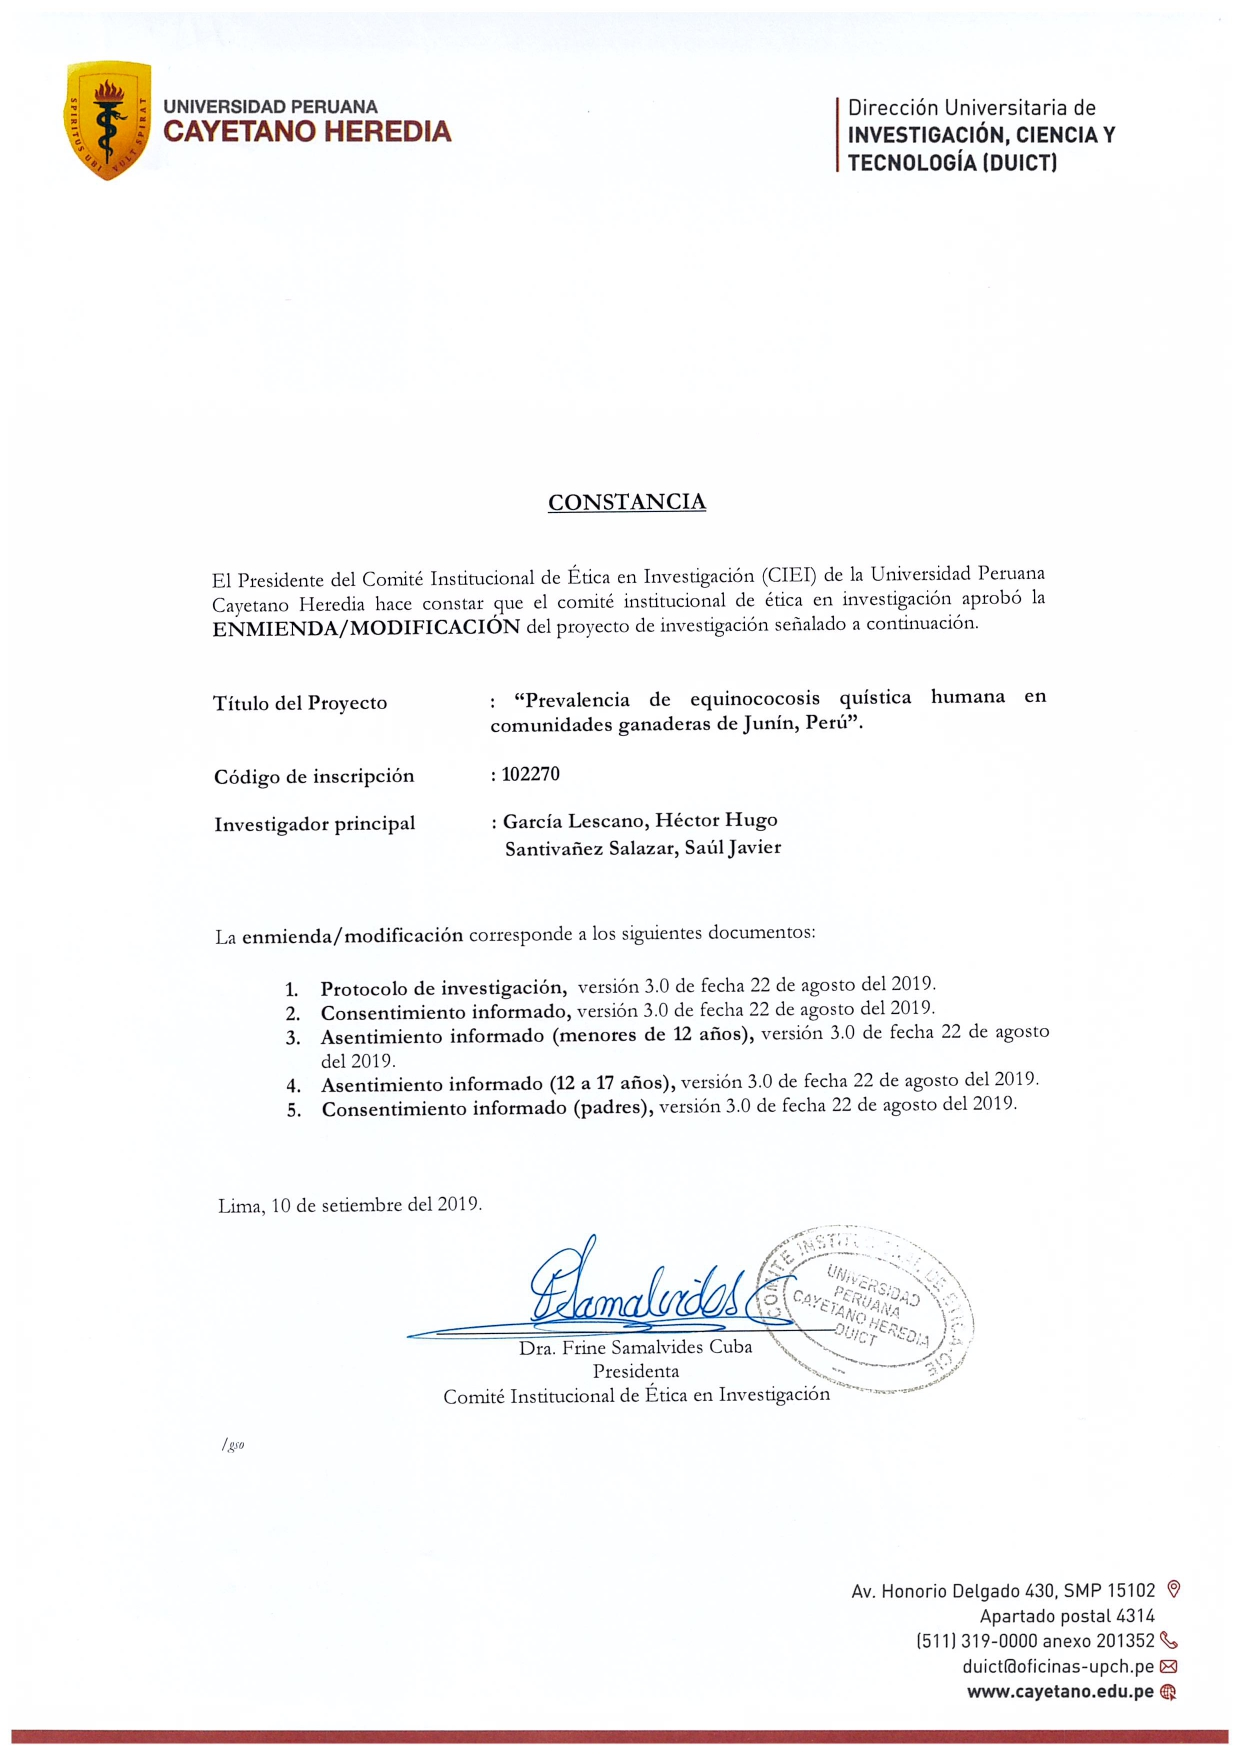
\includegraphics[width=0.5\textwidth]{imagenes/EM_AprobacionEtica.jpg}
    \caption{Carta de Aprobación Ética del Estudio Madre}
    \label{EM_apet}
\end{figure}

%\chapter{Diccionario de variables}\label{DicVar}

%Las variables que conformaron esta base de datos fueron:
%\begin{itemize}[noitemsep,nolistsep]
%    \item paciente: código autogenerado creado para mantener el anonimato del individuo
%    \item sexpac: Sexo del individuo
%    \item edapac: edad del individuo
%    \item ncasa: número de casa
%    \item virit\_wb: Tiene resultado de WB (Wester Blot) en el estudio VIRSEL
%    \item virit\_orden: Orden de participación en el estudio VIRSEL
%    \item virit\_resultado\_wb: Resultado del WB en el estudio VIRSEL
%    \item hycom\_particip: Participación en el estudio HYCOM
%    \item hycom\_orden: Orden de participación en el estudio HYCOM
%    \item hycom\_hid: Diagnostico de Hidatidos en el estudio HYCOM
%    \item hid\_corp: Diagnostico de Hidatidos en Corpacancha
%    \item rando\_edad: Rango de edad
%    \item longitud: Longitud (coordenada) de la casa
%    \item latitud: Latitud (coordenada) de la casa
%    \item distancia\_EsSalud: Distancia de la casa al centro de EsSalud
%\end{itemize}



\chapter{Códigos empleados para el desarrollo de la tesis}\label{CodR}


\begin{figure}[h]
	\centering
	
\includegraphics[width=0.5\textwidth]{imagenes/qr_codigo.png}
	\caption{QR enlazado al repositorio en GITHUB que contiene los códigos trabajados}
\end{figure}
